Es wird  in  Detail  beschrieben,  welche  elektronische Komponenten aus welchem
Grund ausgew\"ahlt worden sind.

% **************************************************************************** %
\subsection{36V Netzteil und Netzeingang}
% **************************************************************************** %

Die  maximale Ausgangsleistung wurde grob berechnet  mit  $\SI{24}{\volt}  \cdot
\SI{3}{\ampere} = \SI{72}{\watt}$.

Da  das  Aufbauen  eines  eigenen  Netzteils  f\"ur  diese  Ausgangsleistung  zu
aufw\"andig und teuer gewesen w\"are, entschieden  wir  uns  f\"ur  ein externes
Netzger\"at dass im Geh\"ause  montiert  werden  kann.  Das  verwendete Netzteil
liefert  \SI{36}{\volt}   und   \SI{75}{\watt}   und   ist   in   der  Abbildung
\ref{fig:circuit:mains-input} als $N_2$ zu sehen.

\begin{figure}[th!]
    \center
    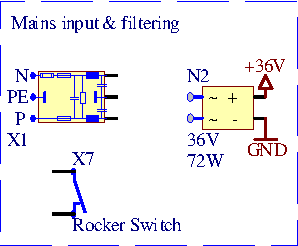
\includegraphics[width=.35\textwidth]{images/circuit/mains-input.pdf}
    \caption{Netzspannung wird gefiltert und auf 36V DC durch ein externes Netzmodul transformiert}
    \label{fig:circuit:mains-input}
\end{figure}

Weiter  wird  eine  Netzeingangs-Steckverbinder  mit integriertem Netzfilter und
Sicherung  verwendet,  was  in der Abbildung  \ref{fig:circuit:mains-input}  als
$X_1$  zu  sehen  ist. Ein auf der R\"uckseit des Geh\"auses montierter Schalter
$X_7$ erlaubt das Ein- und Ausschalten des Endproduktes.

% **************************************************************************** %
\subsection{Spannungsversorgungen}
% **************************************************************************** %

F\"ur die digitale  Logik  werden  die  zwei  Spannungspegel  \SI{5}{\volt}  und
\SI{3.3}{\volt} ben\"otigt. 

\begin{figure}[th!]
    \center
    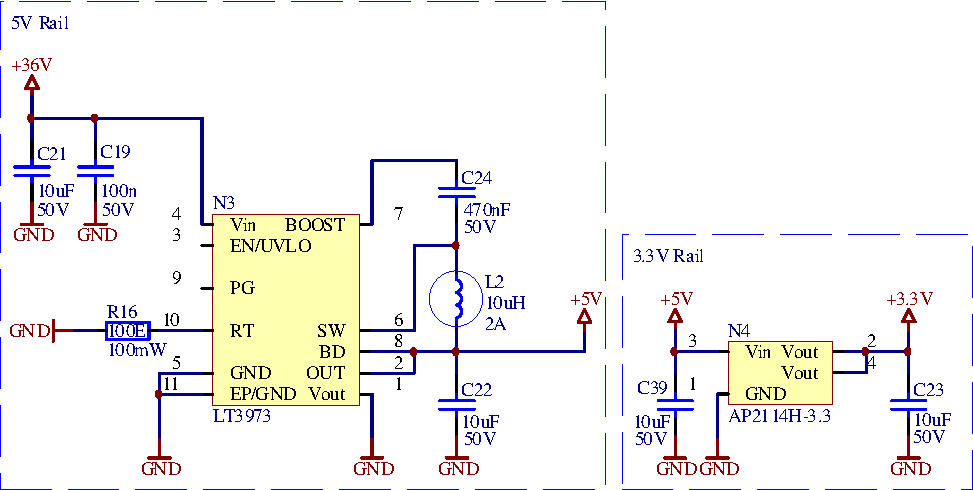
\includegraphics[width=.75\textwidth]{images/circuit/5v-3v-rails.pdf}
    \caption{Speisung f\"ur 5V mittels Abwertswandler (links) und Speisung f\"ur 3.3V mittels Linearregler (rechts)}
    \label{fig:circuit:rails}
\end{figure}

Die  \SI{36}{\volt} vom Netzteil werden mittels eines getakteten  DC-DC-Wandlers
auf \SI{5}{\volt} transformiert,  was  in  der Abbildung \ref{fig:circuit:rails}
vom Bauteil $N_3$ verwirklicht wird.

Die  \SI{5}{\volt}  werden  von  einem  Linearregler $N_4$  auf  \SI{3.3}{\volt}
gestuft.  Ein  Linearregler  wurde  gew\"ahlt damit die \SI{3.3}{\volt} Speisung
m\"oglichst St\"orfrei bleibt.  Somit  wird  verhindert,  dass die DACs und ADCs
verrauscht sind und ungenau messen.

% **************************************************************************** %
\subsection{LT3741}
% **************************************************************************** %

Die  Ausgangsspannung   muss   mindestens   im  Bereich  von  \SI{0}{\volt}  bis
\SI{24}{\volt}  liegen  und   einen  Rippel  kleiner  als  \SI{300}{\milli\volt}
besitzen.  Der  Ausgangsstrom muss mindestens im Bereich von \SI{0}{\ampere} bis
\SI{3.5}{\ampere} liegen  und  einen  Rippel kleiner als \SI{100}{\milli\ampere}
besitzen. Dabei  sollte  die Effizienz bei Volllast mindestens \SI{80}{\percent}
betragen.

Da  das  Endprodukt  schlussendlich  in  Serie  mit  mehreren   Spannungs-  oder
Stromquellen  geschalten  werden  k\"onnte, muss  zus\"atzlich  darauf  geachtet
werden,  dass  der Spannungswandler \emph{leistungsaufnahmef\"ahig}  sein  muss.
Diese Eigenschaft weist  ein  sogenannter  \emph{Synchronwandler}  vor und wurde
zusammen mit den Spannungs-,  Strom-,  und Leistungsanforderungen als prim\"ares
Merkmal f\"ur die Produktsuche eines Wandlers verwendet.

Der LT3741 ist einer der Bauteile,  die  alle  Anforderungen  erf\"ullt.  In der
Abbildung \ref{fig:circuit:buck} ist der Aufbau zu sehen.

\begin{figure}[th!]
    \center
    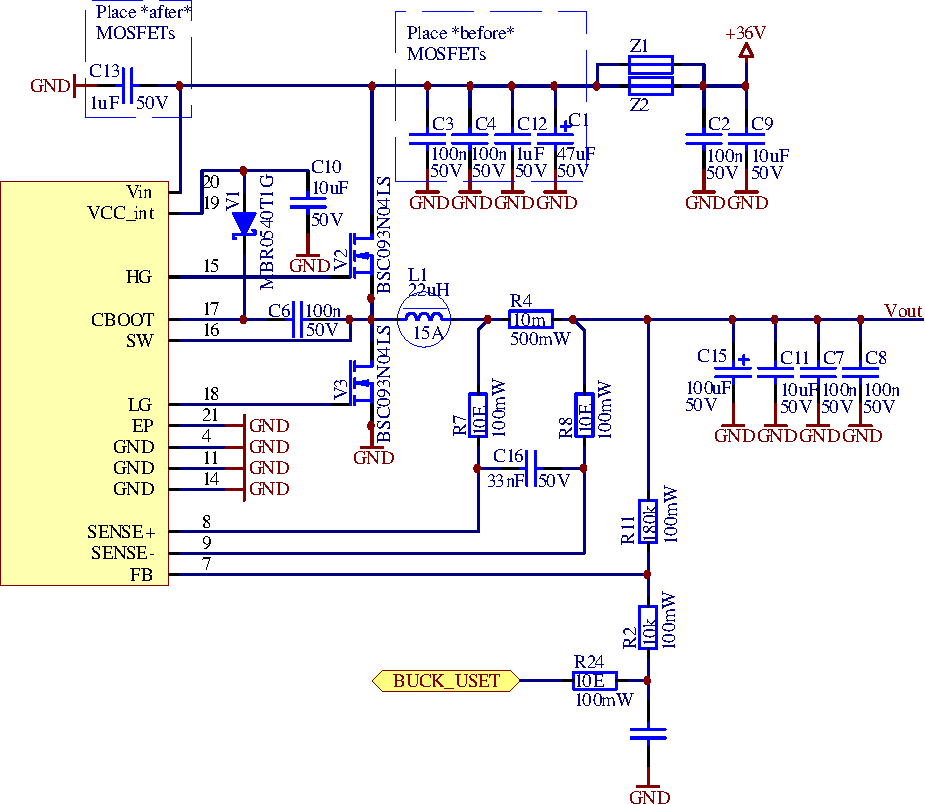
\includegraphics[width=.75\textwidth]{images/circuit/buck.pdf}
    \caption{Herzst\"uck des Projektes: Aufbau des LT3741 CVCC Synchronwandler}
    \label{fig:circuit:buck}
\end{figure}

% **************************************************************************** %
\subsubsection*{St\"utzkondensatoren}
% **************************************************************************** %

Der  LT3741  wird mit \SI{36}{\volt} gespiesen (oben  rechts  in  der  Abbildung
\ref{fig:circuit:buck}).   Da   diese   Schaltung   viel   St\"orung   auf   der
\SI{36}{\volt}    Speisung     verursachen    w\"urde,    werden    verschiedene
Keramikkondensatoren  und  Ferritkerne  verwendet,  um die hochfrequente Signale
m\"oglichst von der Speisung zu eliminieren und somit die anderen Speisungen von
ungewollten St\"orungen zu bewahren.

% **************************************************************************** %
\subsubsection*{Schaltfrequenz}
% **************************************************************************** %

Eine h\"ohere Schaltfrequenz $f_S$ bedeutet eine niedrigere Rippelspannung, aber
eine h\"ohere Verlustleistung. $f_S$ wurde so hoch wie m\"oglich  dimensioniert,
was sich als $\approx \SI{800}{\kilo\hertz}$ herausstellte. In den nachfolgenden
Berechnungen wird aber \SI{1}{\mega\hertz} verwendet.

% **************************************************************************** %
\subsubsection*{Auswahl Spule}
% **************************************************************************** %

Die Spule $L_1$, ersichtlich in der Abbildung \ref{fig:circuit:buck}, wurde  mit
der Formel \ref{eq:circuit:buck:inductor} berechnet,

\begin{equation}
    L_1 = \left( \frac{U_{in} \cdot U_{out} - U_{out}^2}{0.3 \cdot f_S \cdot I_O \cdot U_{in}} \right) = \SI{6}{\micro\henry}
    \label{eq:circuit:buck:inductor}
\end{equation}

wobei  $U_{in}$  die  Eingangsspannung von  \SI{36}{\volt}  ist,  $U_{out}$  die
Ausgangsspannung  bei  gr\"osster   Leistung  ist  (\SI{18}{\volt}),  $f_S$  die
Schaltfrequenz von  \SI{1}{\mega\hertz} ist und $I_o$ der maximale Ausgangsstrom
von \SI{5}{\ampere} ist.

Um den Rippel  noch ein wenig mehr zu gl\"atten, wurde eine gr\"ossere Spule von
\SI{22}{\micro\henry} ausgew\"ahlt.

Der Maximalstrom durch die Spule ist gleich gross wie  der  Strom, der durch den
MOSFET   fliesst   und   wird  mit  der  Formel  \ref{eq:circuit:buck:mosfet_id}
berechnet.  Der  S\"attigungsstrom   wurde   mit   $1.2   \cdot   I_{D_{max}}  =
\SI{6.2}{\ampere}$ berechnet. Es  wurde  nach passende Spulen gesucht, welche in
der Tabelle \ref{tab:circuit:buck:inductor} eingetragen sind.

\begin{table}[th!]
    \begin{center}
        \caption{}
        \label{tab:circuit:buck:inductor}
        \begin{tabular}{lcccc}
            \toprule
            Digikey         & Price (CHF) & Inductance (\SI{}{\micro\henry}) & DCR (\SI{}{\ohm}) & Ohmic Loss (\SI{}{\watt}) \\
            \midrule
            \rowcolor{lightgray}
            732-4237-1-ND   & 8.03        & 22                               & 0.007             & 0.175  \\
            732-2179-1-ND   & 6.4         & 47                               & 0.0335            & 0.8375 \\
            732-2177-1-ND   & 6.4         & 22                               & 0.0146            & 0.365  \\
            \bottomrule
        \end{tabular}
    \end{center}
\end{table}

Unter den Kandidaten ist ganz klar wegen des niedrigen DCRs die Erste,  mit Grau
hervorgehobene Spule die optimalste.

% **************************************************************************** %
\subsubsection*{Auswahl MOSFETs}
% **************************************************************************** %

Die  Bauteile  $V_1$  und  $C_6$  bilden  zusammen  mit  dem  MOSFET  $V_2$  ein
High-Side-Schalter. Im Gegensatz zu einem nicht-synchronen Schaltregler befindet
sich  an  der Stelle wo normalerweise eine Freilaufdiode sein sollte ein zweiter
MOSFET $V_3$. Dieser erm\"oglicht  eine  Spannungsregelung in der gegengesetzten
Richtung -- sprich, sie erm\"oglicht eine Leistungsaufnahme, was, wie oben schon
erw\"ant wurde, kritisch ist.

Bei  der  Auswahl von passenden MOSFETs sind die  Parameter  $Q_G$  (Total  Gate
Charge),  $R_{DS_{(on)}}$  (On-Resistance),  $Q_{GD}$  (Gate to  Drain  Charge),
$Q_{GS}$ (Gate to Source  Charge),  $R_G$  (Gate Resistance), sowie $U_{GS}$ und
$U_{DS}$, $I_{D_{max}}$ und $U_{GS_{THR}}$ kritische Parameter.

Der  maximale  Drain-Strom  kann mit der Formel  \ref{eq:circuit:buck:mosfet_id}
berechnet werden

\begin{equation}
    I_{D_{max}} = I_O + \left( \frac{U_{in} \cdot U_{out} - U_{out}^2}{2 \cdot f_S \cdot L \cdot U_{in}} \right) = \SI{5.2}{\ampere}
    \label{eq:circuit:buck:mosfet_id}
\end{equation}

wobei $I_O$ der maximale Ausgangsstrom  von  \SI{5}{\ampere}  ist,  $U_{in}$ die
Eingangsspannung von  \SI{36}{\volt}  ist,  $U_{out}$  die  Ausgangsspannung bei
gr\"osster  Leistung  ist   (\SI{18}{\volt}),   $f_S$   die  Schaltfrequenz  von
\SI{1}{\mega\hertz}  ist  und  $L$  die  Spule  von  \SI{22}{\micro\henry}  ist.

$U_{DS}$  wurde   h\"oher   gew\"ahlt   als   die   Eingangsspannung  $U_{in}  =
\SI{36}{\volt}$.

Die maximale  Gate-Spannung  $U_{GS}$  betr\"agt  \SI{5}{\volt}.  Da  der LT3741
w\"ahrend  dem Aufstartvorgang Steuersignale knapp unter \SI{3}{\volt}  liefert,
muss  die  Gate-Threshold-Spannung  $U_{GS_{THR}}$  kleiner   als  \SI{2}{\volt}
gew\"ahlt werden.

Leistungsverluste der MOSFETs sind einerseits verbunden mit ohmsche  Verluste --
abh\"angig  von  $R_{DS_{(on)}}$  --  sowie   verbunden  mit  Schaltverluste  --
abh\"angig von $Q_{GS}$ und $Q_{GD}$.

Der    Leistungsverlust    im    High-Side   MOSFET   kann   mit   der    Formel
\ref{eq:circuit:buck:mosfet_ploss} approximiert werden

\begin{multline}
    P_{LOSS} = (\textrm{ohmic loss}) + (\textrm{transission loss}) \\
             \approx \left( I_O^2 \cdot R_{DS_{(on)}} \cdot \rho_T \right)
                    + \left( \frac{U_{in} \cdot I_O}{\SI{5}{\volt}} \cdot \left(Q_{GD} + Q_{GS} \right) \cdot \left( 2 \cdot R_G + R_{PU} + R_{PD} \right) \cdot f_S \right) \\
    \label{eq:circuit:buck:mosfet_ploss}
\end{multline}

wobei $\rho_T$ ein temperaturabh\"angiger  Parameter  vom On-Resistance ist. Bei
\SI{70}{\celsius} betr\"agt $\rho_T \approx 1.3$. $R_{PD}$ und $R_{PU}$ sind die
Ausgangsimpedanzen   vom   LT3741   und   betragen   \SI{1.3}{\ohm}   respektive
\SI{2.4}{\ohm}.

Der  Low-Side MOSFET sollte einen m\"oglichst kleinen $R_{DS_{(on)}}$ haben  und
ein    Total-Gate-Charge    $Q_C    \leq    \SI{30}{\nano\coulomb}$    besitzen.

Ein  weiterer Verlust sind die Schaltverl\"uste der internen  MOSFET-Treiber  im
LT3741. Die Total Gate Charge $Q_C$ muss  w\"ahrend  jedem  Zyklus  geladen  und
wieder   entladen   werden.   Diese   Verl\"uste   k\"onnen   mit   der   Formel
\ref{eq:circuit:buck:switching_loss} berechnet werden,

\begin{equation}
    P_{LOSS\_LDO} \approx \left( (U_{in} - \SI{5}{\volt} \right) \cdot \left( Q_{GLG} + Q_{GHG} \right) \cdot f_S
    \label{eq:circuit:buck:switching_loss}
\end{equation}

wobei $G_{GLG}$ die  Low-Side  Gate-Charge $G_C$ ist und $G_{GHG}$ die High-Side
Gate-Charge ist.

In  der  Tabelle  \ref{tab:circuit:buck:mosfet}  sind  verschiedene MOSFET-typen
aufgelistet, die in den oben genannten Parametern passen. Dabei wurde $P_{LOSS}$
und $P_{LOSS\_LDO}$ f\"ur jeden Kandidaten berechnet.

\begin{table}[th!]
    \begin{center}
        \caption{}
        \label{tab:circuit:buck:mosfet}
        \begin{tabular}{cccccccccc}
            \toprule
            $R_{DS_{(on)}}$ & $Q_{GD}$ & $Q_{GS}$ & $R_G$ & $U_{GS_{THR}}$ & Ohmic Loss & Transision Loss & Total Loss & Drive Loss \\
            \midrule
            0.0032          & 4        & 2.5      & 0.4   & 2.5            & 0.104      & 1.0296          & 1.1336     & 0.806 \\
            0.0039          & 7        & 9        & 2.4   & 3.3            & 0.12675    & 4.8384          & 4.96515    & 1.984 \\
            0.0042          & 7        & 9        & 2.4   & 3.3            & 0.1365     & 4.8384          & 4.9749     & 1.984 \\
            0.008           & 2        & 4.5      & 3     & 2              & 0.26       & 2.2464          & 2.5064     & 0.558 \\
            0.0067          & 5.3      & 3.9      & 1.5   & 1              & 0.21775    & 2.18592         & 2.40367    & 0.7998 \\
            \rowcolor{lightgray}
            0.0093          & 2        & 4.9      & 1     & 2              & 0.30225    & 1.39104         & 1.69329    & 1.488 \\
            0.019           & 8        & 4        & 1.3   & 2              & 0.6175     & 2.6784          & 3.2959     & 1.798 \\
            0.0095          & 7.5      & 6        & 1     & 3              & 0.30875    & 2.7216          & 3.03035    & 1.736 \\
            \bottomrule
        \end{tabular}
    \end{center}
\end{table}

Vergleicht  man  \emph{Total  Loss}  und  \emph{Drive Loss}, w\"ahre der oberste
MOSFET  geeigneter. Aus Kostengr\"unden und  generell  schlechter  Dokumentation
wurde  aber  der   n\"achst  bessere  MOSFET  gew\"ahlt  --  hier  mit  hellgrau
hervorgehoben.

Es  wird  f\"ur  den  High-Side  MOSFET wie auch f\"ur den Low-Side  MOSFET  der
gleiche Typ verwendet.

% **************************************************************************** %
\subsubsection*{Spannungs- und Strommessung}
% **************************************************************************** %

Der  LT3741  ist   sowohl   Spannungsgesteuert   wie  auch  Stromgesteuert.  Der
Spannungsteiler $R_{11} \parallel  R_2$  erlaubt das Messen der Ausgangsspannung
und ein Shunt-Widerstand $R_4$ erm\"oglicht die genaue \"Uberwachung des Stromes
durch  die  Spule  $L_1$. Der Widerstand $R_4$  wurde  so  gew\"ahlt  damit  der
maximale Ausgangsstrom maximal \SI{5}{\ampere} betragen kann.

Strom\"uberwachung   ist  sehr  wichtig  bei  einer  solchen  Aufgabe   wo   die
Ausgangsspannung  sich  konstant  \"andert.  Sie erlaubt  genauer  vorhersebares
Verhalten der Spannungs\"anderung am Ausgang -- \"Uberschiessen der Sollspannung
und   extreme   Stromspitzen   in   der   Spule   k\"onnen   vermieden   werden.

Weiter   kann   ein   Stromgesteuerter   Regler  auch  als   Konstantstromquelle
funktionieren. Diese Eigenschaft  ist  vorallem  dann  von  Bedeutung  wenn  der
Arbeitspunkt  sich  im  ``steilen''  bereich  der   UI-Kennlinie  des  PV-Moduls
befindet.

Die   Widerst\"ande   $R_2$   und    $R_{11}$    wurden    nach    der    Formel
\ref{eq:circuit:buck:feedback_resistors}      dimensioniert      damit       die
Ausgangsspannung maximal \SI{23}{\volt} betr\"agt.

\begin{equation}
    U_{out} = \SI{1.21}{\volt} \left( 1 + \frac{R_{11}}{R_2} \right)
    \label{eq:circuit:buck:feedback_resistors}
\end{equation}

Die Ausgangsspannung kann  danach  durch Anheben der Bezugsspannung $BUCK\_USET$
nach der  Formel \ref{eq:circuit:buck:uset} ver\"andert werden. 

\begin{equation}
    U_{out} = (\SI{1.21}{\volt} - BUCK\_USET) \cdot \frac{R_{11} + R_2}{R_2}
    \label{eq:circuit:buck:uset}
\end{equation}

Wobei $BUCK\_USET$ die analoge Spannung vom ersten DAC ist.

In der Abbildung \ref{fig:circuit:buck:uset}  ist  die dazugeh\"orige Schaltung.

\begin{figure}[th!]
    \center
    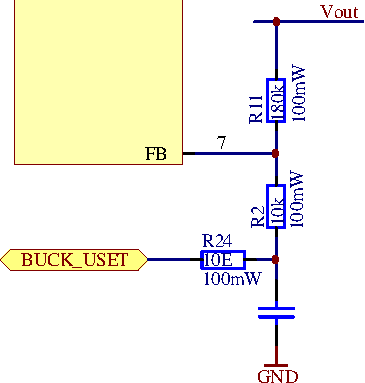
\includegraphics[width=.35\textwidth]{images/circuit/buck-uset.pdf}
    \caption{Einstellung der Ausgangsspannung durch \"Anderung der Bezugsspannung im Feedback-Loop mittels einer analogen Steuerspannung von 0V bis 1.21V}
    \label{fig:circuit:buck:uset}
\end{figure}

Analog zur Ausgangsspannung kann durch anlegen einer analogen Spannung  zwischen
\SI{0}{\volt}  und  \SI{1.5}{\volt}  am  Eingang   CTRL1   direkt  der  maximale
\emph{Durchschnittsstrom}   durch   die  Spule  $L_1$  und  somit  der  maximale
Ausgangsstrom eingestellt werden.

\begin{figure}[th!]
    \center
    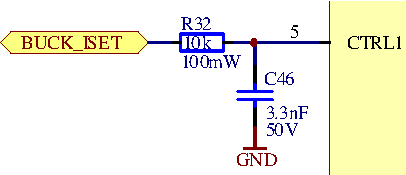
\includegraphics[width=.4\textwidth]{images/circuit/buck-iset.pdf}
    \caption{Einstellung des Maximalstroms mittels einer analogen Steuerspannung von 0V bis 1.5V}
    \label{fig:circuit:buck:iset}
\end{figure}

Die Abbildung \ref{fig:circuit:buck:iset} zeigt  die  dazugeh\"orige  Schaltung.
Der   maximale  durchschnittliche  Ausgangsstrom  $I_o$  wird  mit  der   Formel
\ref{eq:circuit:buck:output_current} berechnet

\begin{equation}
    I_o = \frac{U_{CTRL1}}{30 \cdot R_4}
    \label{eq:circuit:buck:output_current}
\end{equation}

wobei $U_{CTRL1}$ die  analoge  Steuerspannung vom zweiten DAC ist und $R_4$ der
\SI{10}{\milli\ohm}    Shunt-Widerstand    ist,   welcher   in   der   Abbildung
\ref{fig:circuit:buck} zu sehen ist.

Damit der Mikrocontroller angemessene Steuerspannungen  generieren kann, braucht
er die Ausgangsspannung und den Ausgangsstrom zu messen.

Die   Ausgangsspannung   wird   mittels   der   Schaltung   in   der   Abbildung
\ref{fig:circuit:buck:umeas} gemessen. Die Widerst\"ande $R_{12}$  und  $R_{15}$
wurden  so  dimensioniert  damit  die  Spannung  $BUCK\_UMEAS$  in  den  Bereich
\SI{0}{\volt} bis \SI{1.5}{\volt} skaliert ist.

\begin{figure}[th!]
    \center
    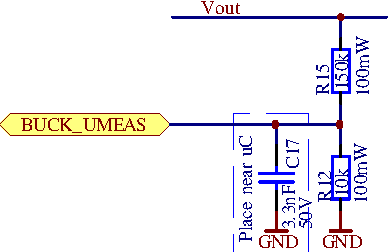
\includegraphics[width=.45\textwidth]{images/circuit/buck-umeas.pdf}
    \caption{Messen der Ausgangsspannung}
    \label{fig:circuit:buck:umeas}
\end{figure}

Der  Ausgangsstrom  wird  mittels  einem  Shunt-Widerstand  $R_5$  differentiell
gemessen.  Die  Schaltung dazu  ist  in  Abbildung  \ref{fig:circuit:buck:imeas}
dargestellt.

\begin{figure}[th!]
    \center
    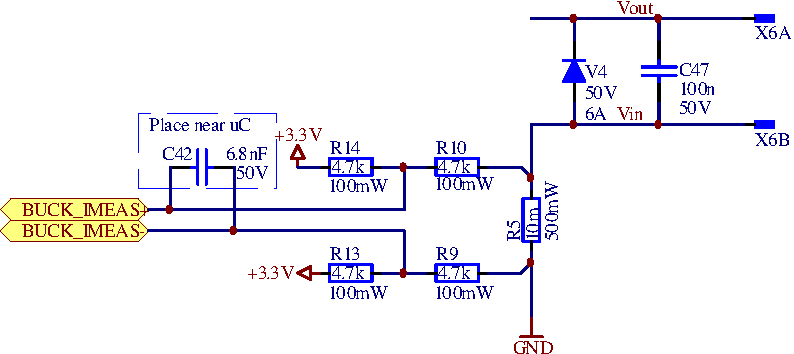
\includegraphics[width=.85\textwidth]{images/circuit/buck-imeas.pdf}
    \caption{Messen des Ausgangsstromes}
    \label{fig:circuit:buck:imeas}
\end{figure}

Der  Mikrocontroller verf\"ugt \"uber einer differentiellen ADC mit  eingebauter
Vorverst\"arkung.

% **************************************************************************** %
\subsubsection*{Ausgang}
% **************************************************************************** %

Die Ausgangsspannung wird \"uber zwei  Bananenstecker  $X_{6A}$ und $X_{6B}$ ans
\"Aussere    des    Geh\"auses     gef\"uhrt.     Die    Ausgangsspannung    ist
verpolungsgesch\"utzt mit der Diode $V_4$.

\begin{figure}[th!]
    \center
    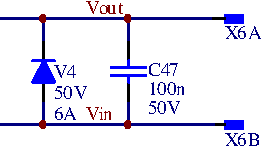
\includegraphics[width=.35\textwidth]{images/circuit/output-connectors.pdf}
    \caption{Verpolungsschutz am Ausgang}
    \label{fig:circuit:output}
\end{figure}

Damit die ADCs und DACs  m\"oglichst  genau messen und m\"oglichst in Full-Range
betrieben    werden   k\"onnen,   wird   eine   externe   Referenzspannung   von
\SI{1.5}{\volt}    verwendet     (siehe    Abbildung    \ref{fig:circuit:vref}).

\begin{figure}[th!]
    \center
    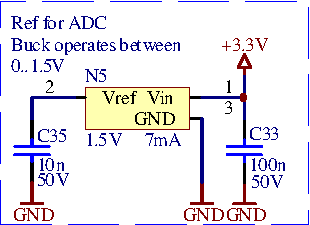
\includegraphics[width=.4\textwidth]{images/circuit/vref.pdf}
    \caption{1.5V Referenzspannung um die ADCs m\"oglichst in Full-Range betreiben zu k\"onnen}
    \label{fig:circuit:vref}
\end{figure}

% **************************************************************************** %
\subsubsection*{Enable und UVLO}
% **************************************************************************** %

Der \emph{Enable}-Eingang des LT3741 wird einerseits vom Mikrocontroller mit dem
$BUCK\_EN$ Signal ein- und ausgeschalten, anderseits wird er Enable-Eingang auch
mit vorrang in  Hardware  ausgeschalten, falls die \SI{36}{\volt} Spannung unter
$\approx  \SI{25}{\volt}$  sinken  w\"urde. Dies erlaubt ein kontrolliertes  und
vorhersehbares Verhalten des LT3741 w\"ahrend Ein-  und Ausschaltvorg\"angen des
Endproduktes.  Die  Schaltung  dazu  ist in der Abbildung \ref{fig:circuit:uvlo}
ersichtlich.

\begin{figure}[th!]
    \center
    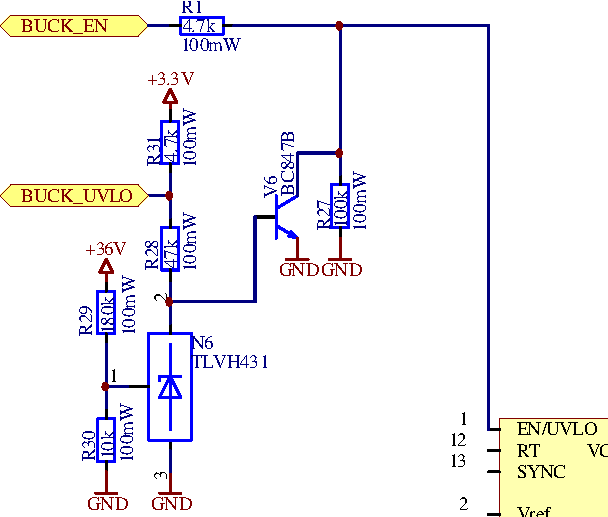
\includegraphics[width=.6\textwidth]{images/circuit/uvlo.pdf}
    \caption{Under-Voltage Lock-Out (UVLO) erm\"oglicht ein kontrolliertes Ein- und Ausschalten des Reglers}
    \label{fig:circuit:uvlo}
\end{figure}

Im Falle einer Unterspannung  wechselt  $N_6$  in den sperrenden Zustand \"uber,
der  Transistor $V_6$ beginnt zu leiten, und der  Enable-Eingang  wird  auf  Low
gezogen.  Die  Spannung  an  $BUCK\_UVLO$  triggert  beim  Mikrocontroller   ein
Interrupt.

% **************************************************************************** %
\subsection{Druck-Drehtaster}
% **************************************************************************** %

\begin{figure}[th!]
    \center
    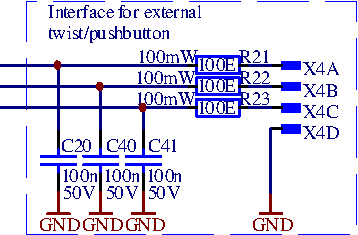
\includegraphics[width=.4\textwidth]{images/circuit/pushbutton.pdf}
    \caption{Drehdruckknopf}
    \label{fig:circuit:pushbutton}
\end{figure}

